\documentclass[tikz,border=2pt]{standalone}
\usepackage{amsmath,amssymb}
\usepackage{tikz}
\usetikzlibrary{arrows.meta}

\begin{document}
% i sits one unit up the imaginary axis; multiplying by i rotates by a quarter turn, so two
% such rotations give i^2 = -1.
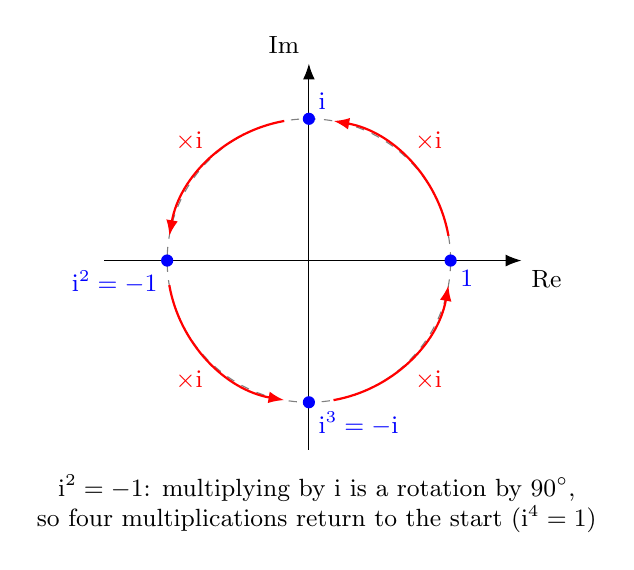
\begin{tikzpicture}[every node/.style={font=\small}, >={Latex[length=2mm]}]
	\draw[->] (-2.6,0) -- (2.7,0) node[below right] {$\mathrm{Re}$};
	\draw[->] (0,-2.4) -- (0,2.5) node[above left] {$\mathrm{Im}$};
	\draw[gray, dashed] (0,0) circle (1.8);
	\fill[blue] (1.8,0) circle (2.2pt) node[below right] {$1$};
	\fill[blue] (0,1.8) circle (2.2pt) node[above right] {$\mathrm{i}$};
	\fill[blue] (-1.8,0) circle (2.2pt) node[below left] {$\mathrm{i}^2=-1$};
	\fill[blue] (0,-1.8) circle (2.2pt) node[below right] {$\mathrm{i}^3=-\mathrm{i}$};
	\draw[red, thick, ->] (10:1.8) arc (10:80:1.8);
	\node[red, font=\small] at (45:2.15) {$\times \mathrm{i}$};
	\draw[red, thick, ->] (100:1.8) arc (100:170:1.8);
	\node[red, font=\small] at (135:2.15) {$\times \mathrm{i}$};
	\draw[red, thick, ->] (190:1.8) arc (190:260:1.8);
	\node[red, font=\small] at (225:2.15) {$\times \mathrm{i}$};
	\draw[red, thick, ->] (280:1.8) arc (280:350:1.8);
	\node[red, font=\small] at (315:2.15) {$\times \mathrm{i}$};
	\node[anchor=north, align=center] at (0.1,-2.6) {$\mathrm{i}^2=-1$: multiplying by $\mathrm{i}$ is a rotation by $90^\circ$,\\ so four multiplications return to the start ($\mathrm{i}^4=1$)};
\end{tikzpicture}
\end{document}
